\section{Software implementering}

Efter designfasen er software brudt så meget ned at det er lige til at programmerer.
Programmeringen er sket ud fra de klassediagrammer som blev udviklet i applikationsmodellen.
Da implementeringen giver en endnu større detaljegrad bliver klassediagrammerne også opdateret til statiske klassediagrammer. De er vist i figur \ref{fig:PC_class_static}, figur \ref{fig:CSS_hovedenhed_class_static} og figur \ref{fig:X10_modtager_Class_Static}.

Kildekode for alt software kan findes på vedlagte CD under mappen ''SW Kildekode''.

\begin{figure}[htb]
  \centering
  {
    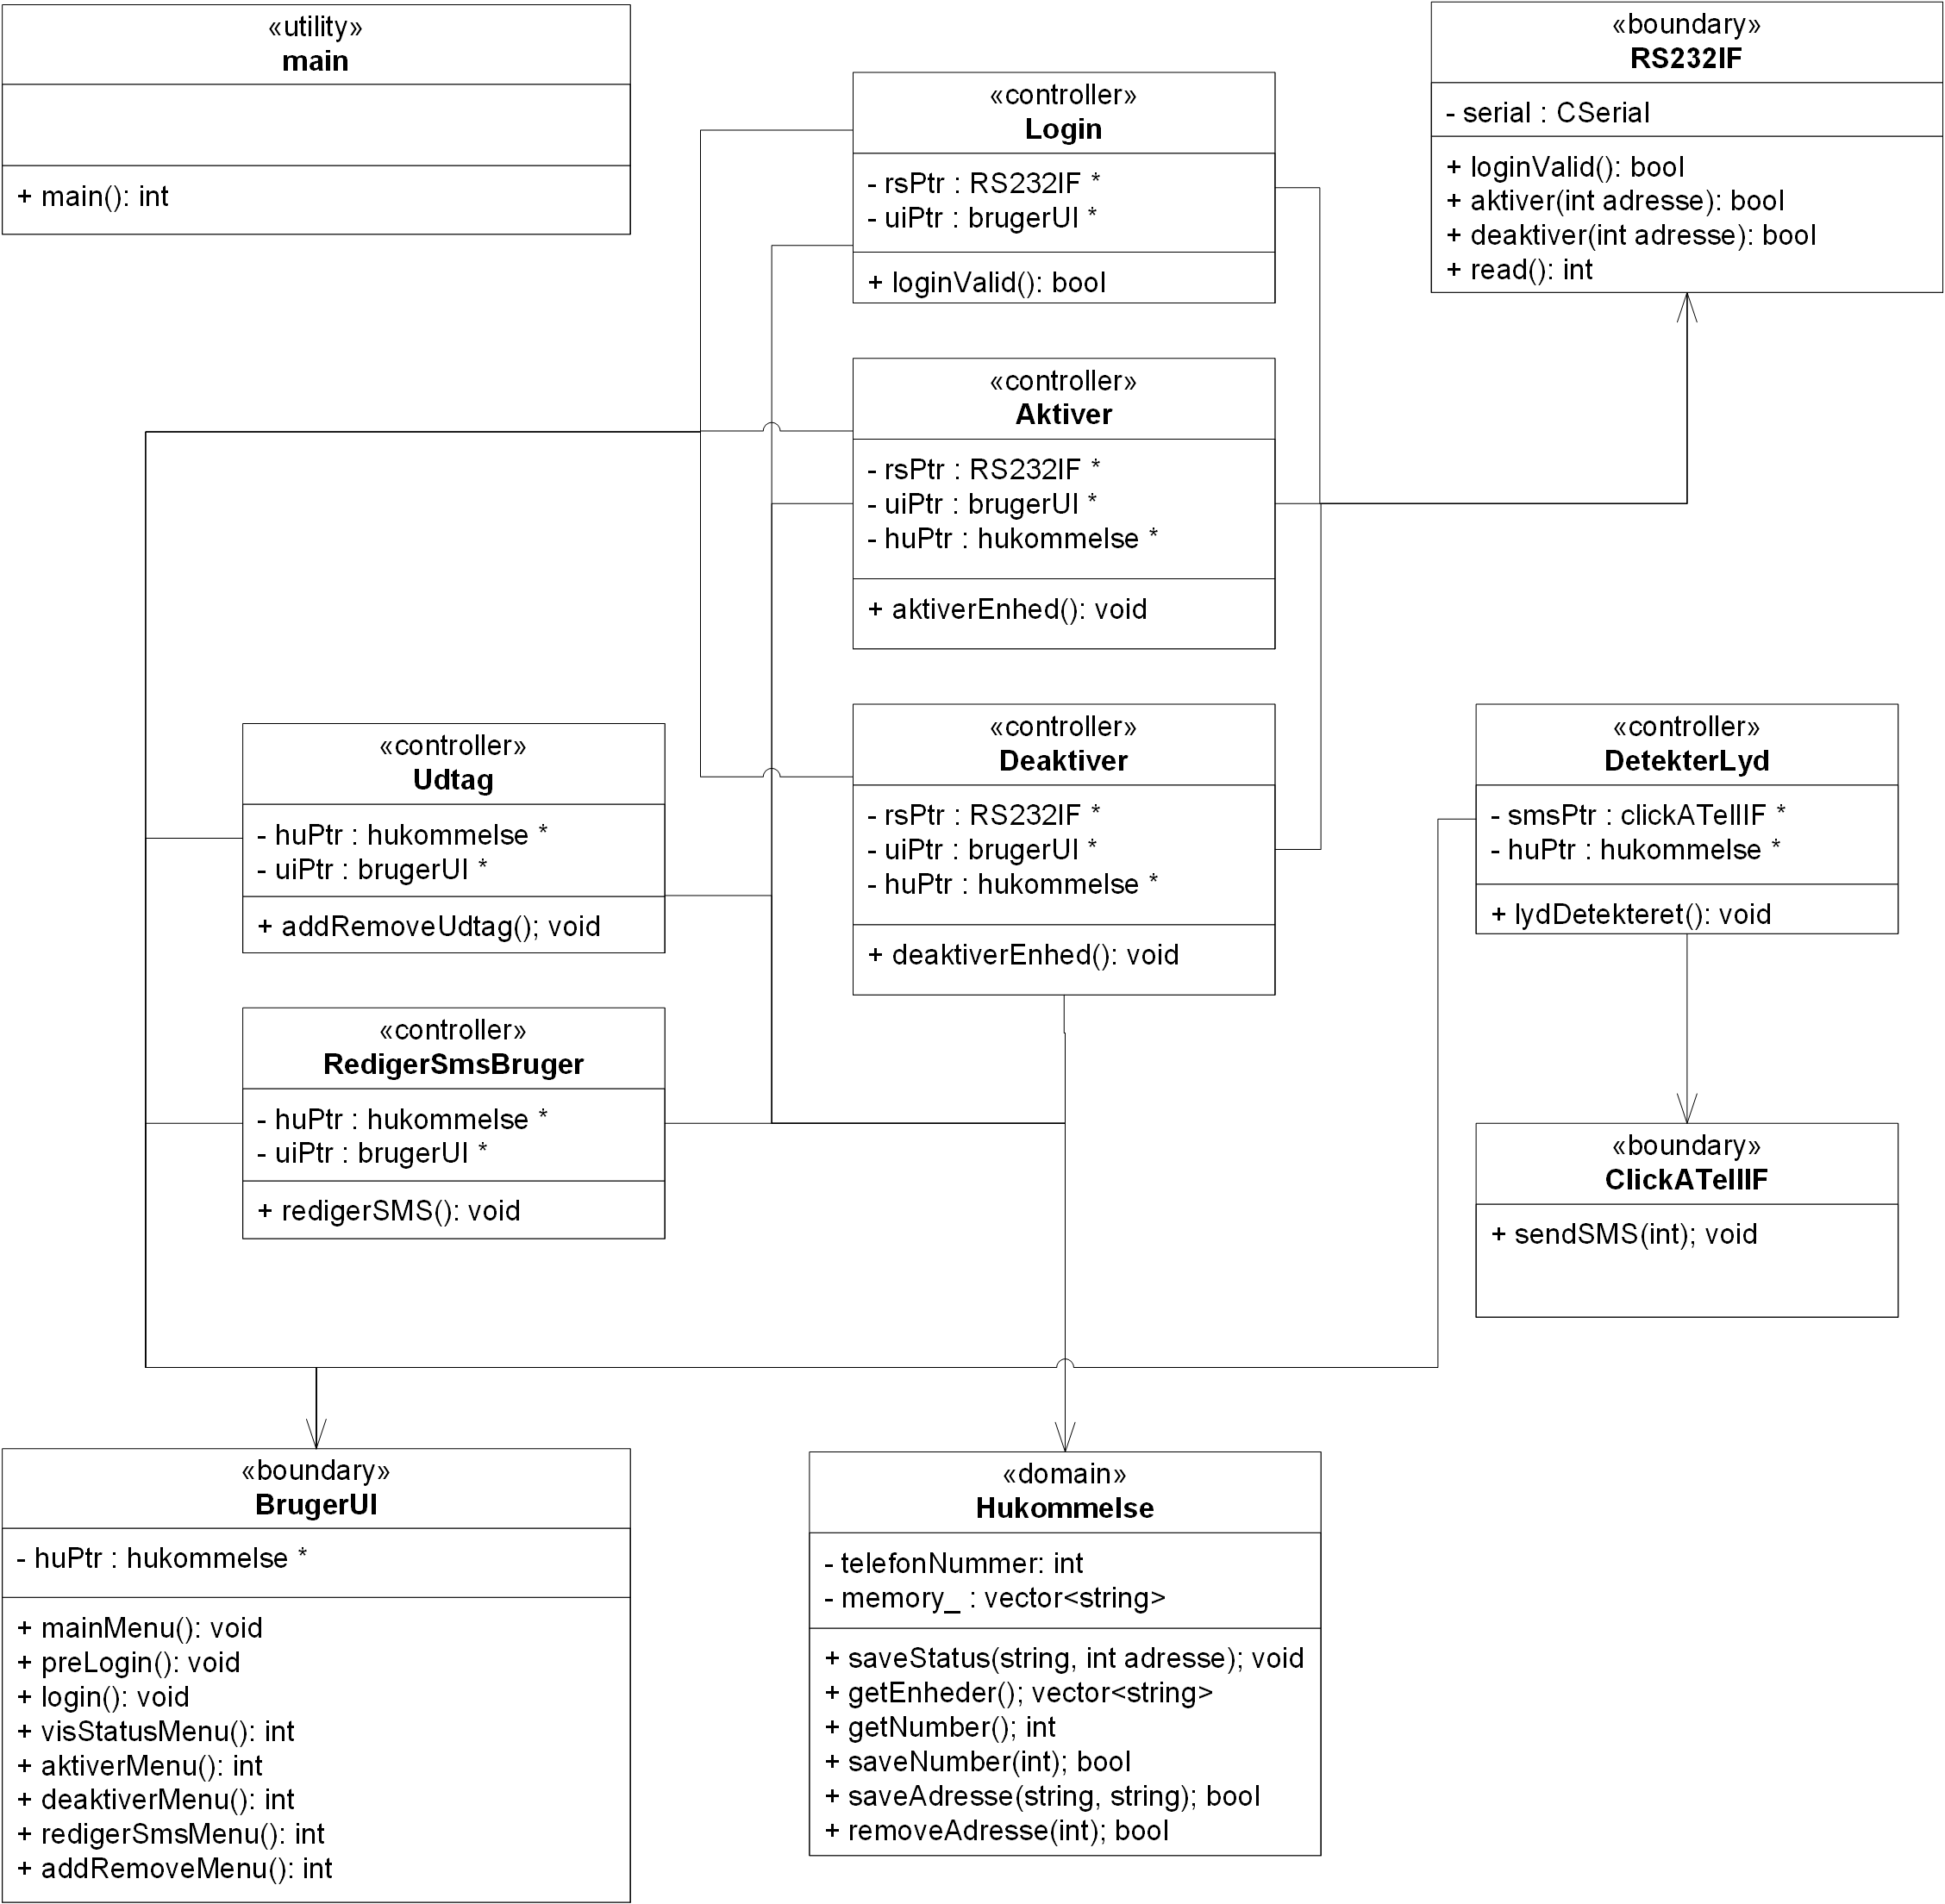
\includegraphics[width=\textwidth]	
      {billeder/uml/PC_Class_static}
  }
  \caption{Statisk klassediagram for PC}
  \label{fig:PC_class_static}
\end{figure}

\begin{figure}[htb]
  \centering
  {
    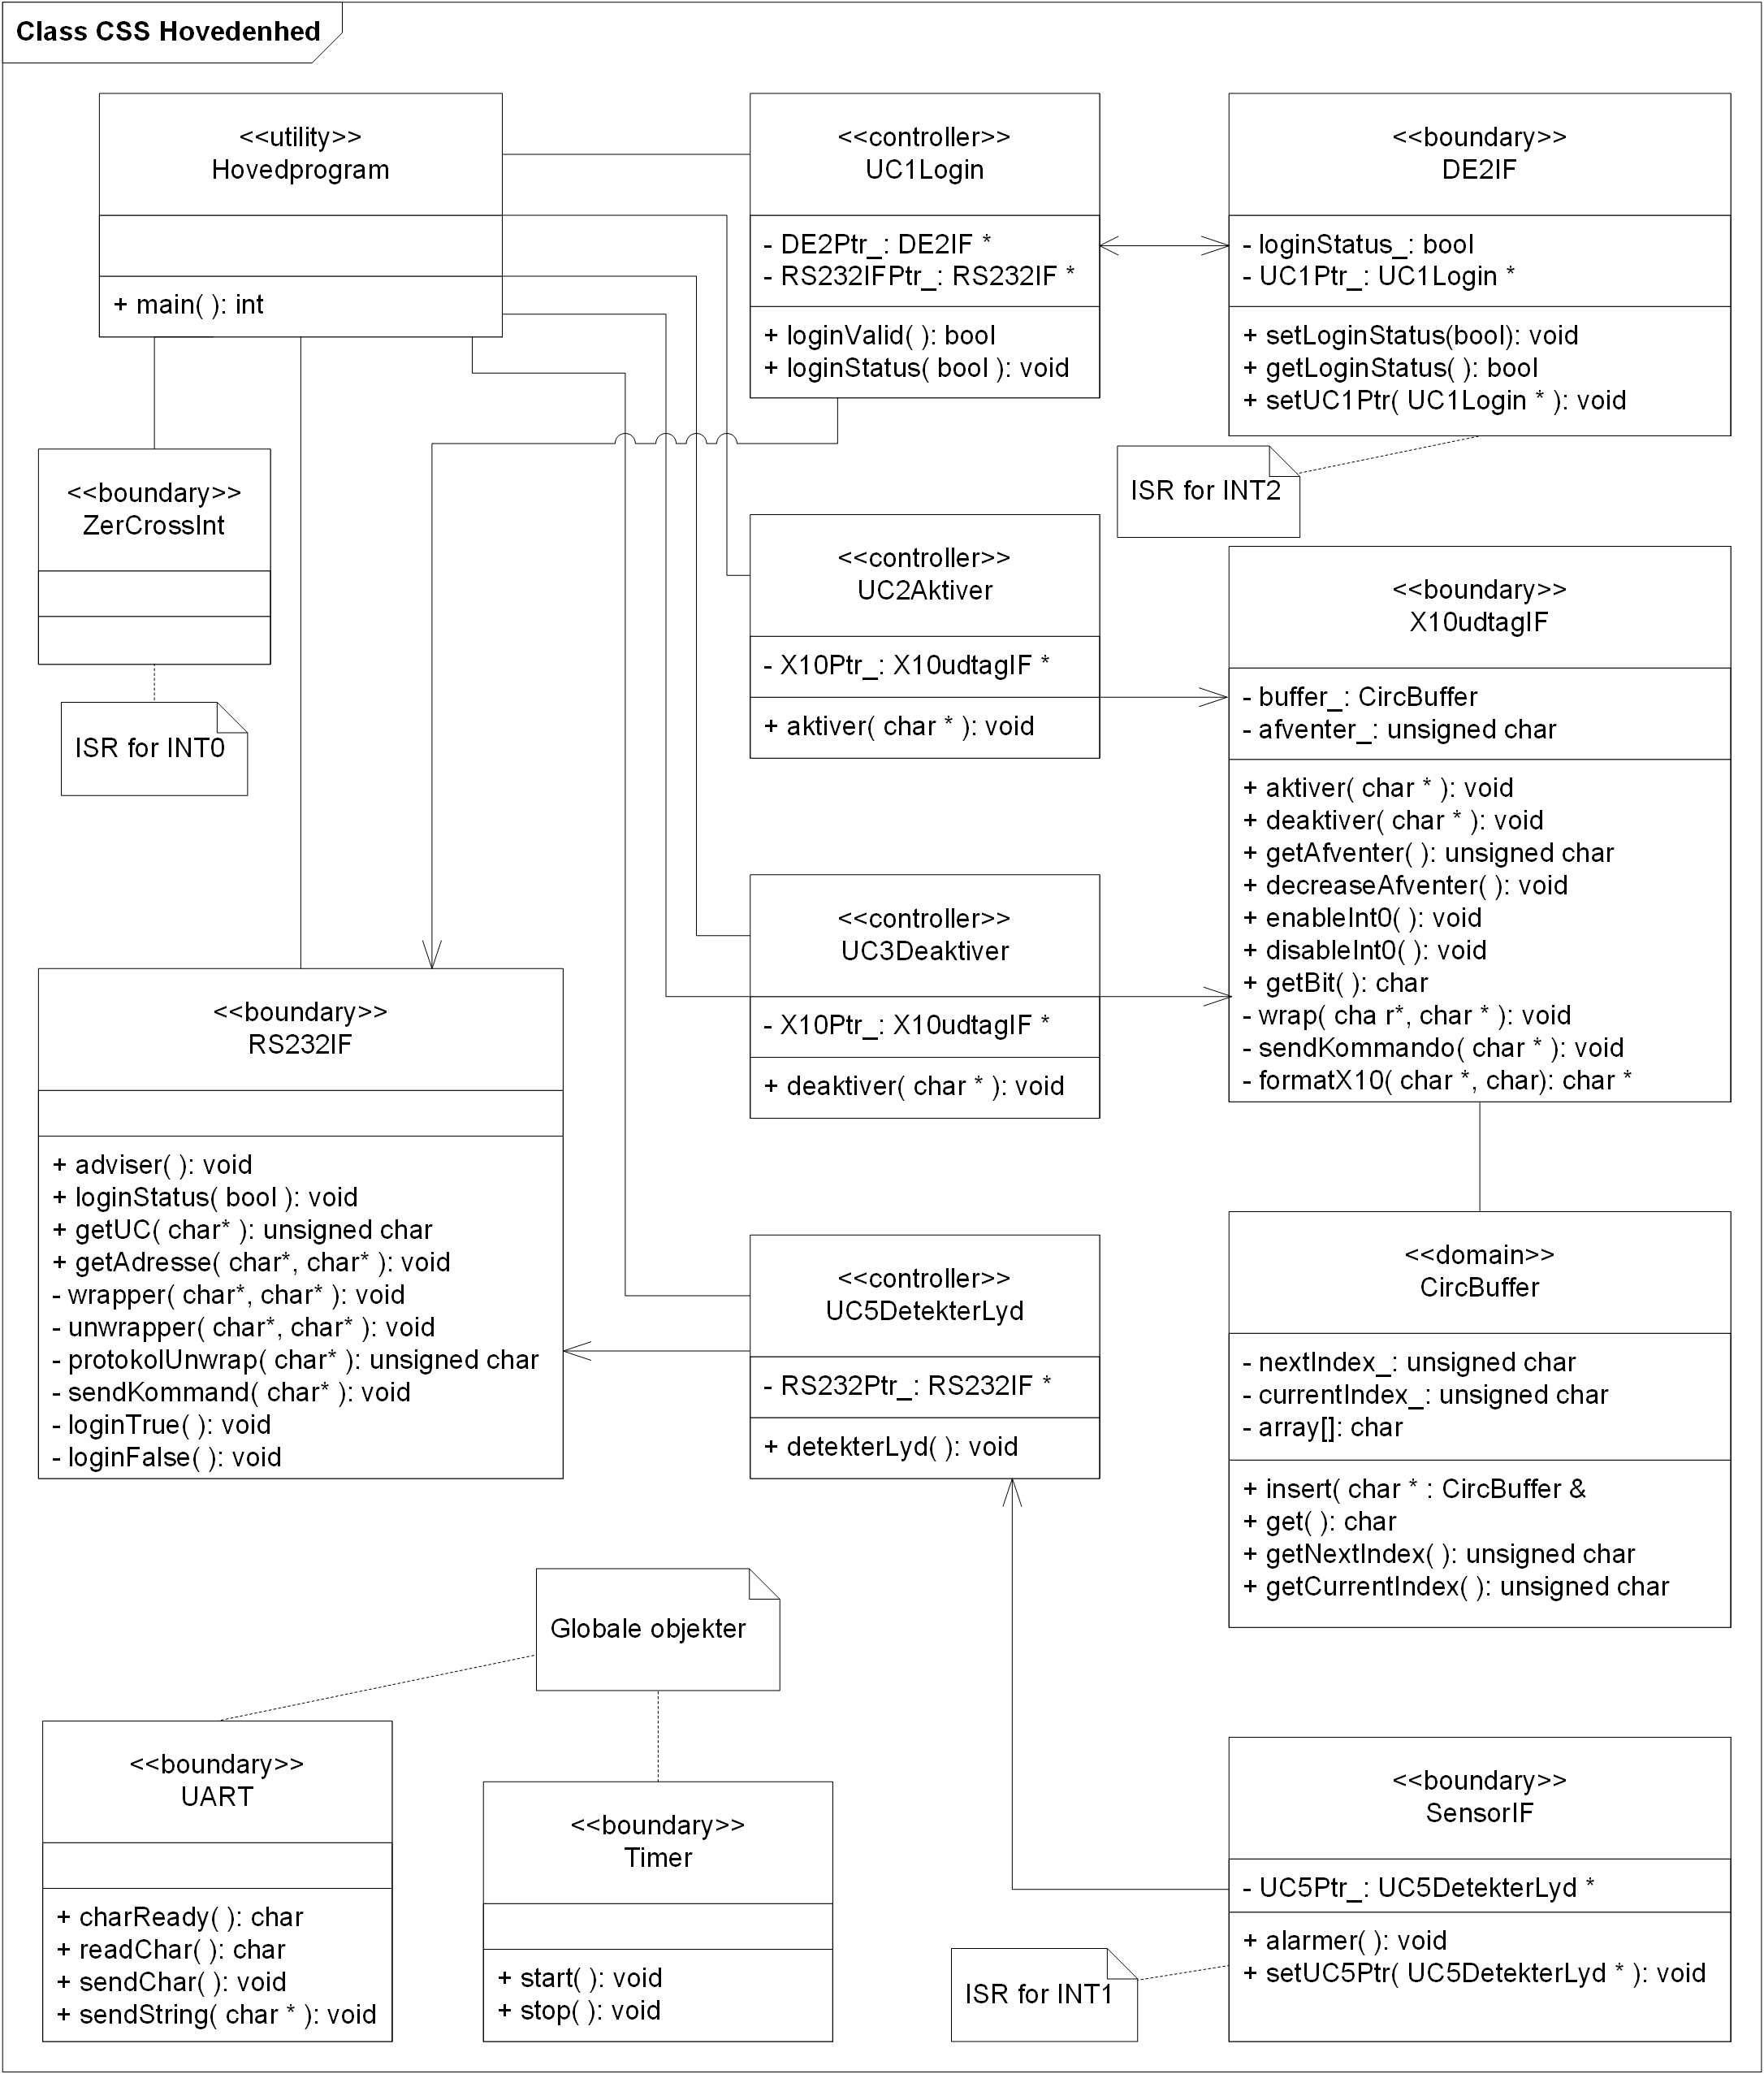
\includegraphics[width=\textwidth]	
      {billeder/uml/CSS_hovedenhed_Class_Static}
  }
  \caption{Statisk klassediagram for CSS-hovedenhed}
  \label{fig:CSS_hovedenhed_class_static}
\end{figure}

\begin{figure}[htb]
  \centering
  {
    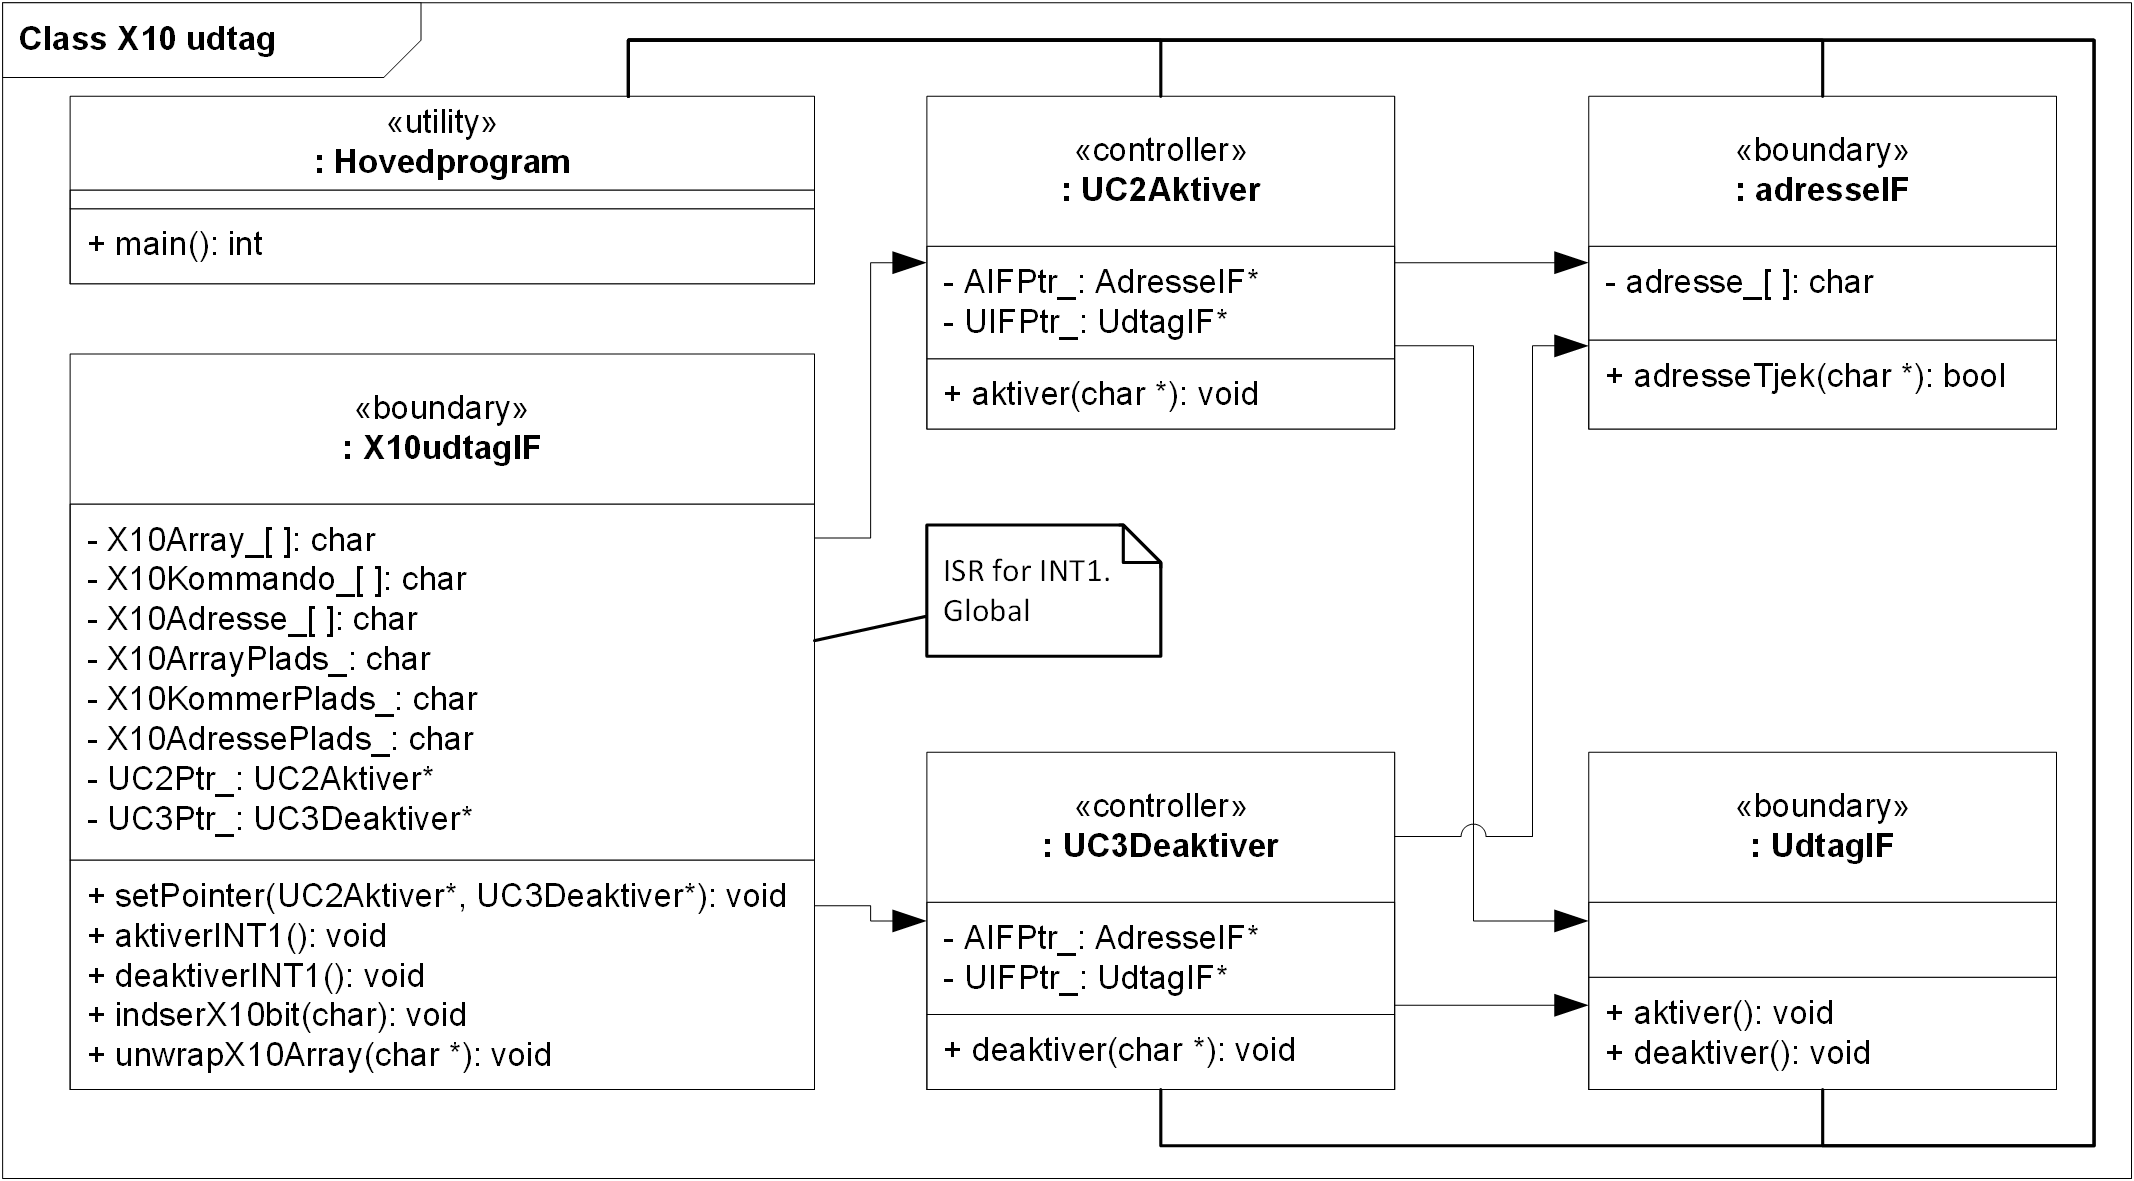
\includegraphics[width=\textwidth]	
      {billeder/uml/X10_modtager_Class_Static}
  }
  \caption{Statisk klassediagram for X10-udtag}
  \label{fig:X10_modtager_Class_Static}
\end{figure}
